%%%
\section{Revising OpenStack\label{sec:leveraging-openstack}}

OpenStack \cite{openstack} is an open-source project that aims at developing a complete CC management system. Its architecture is comparable with the
reference architecture previously described (see Figure~\ref{fig:openstack}). Two kinds of nodes compose an OpenStack infrastructure:~compute and
controller nodes. The former are dedicated to the hosting of VMs while the latter are in charge of executing the OpenStack services.

\begin{figure}[htbp]
        \centering
        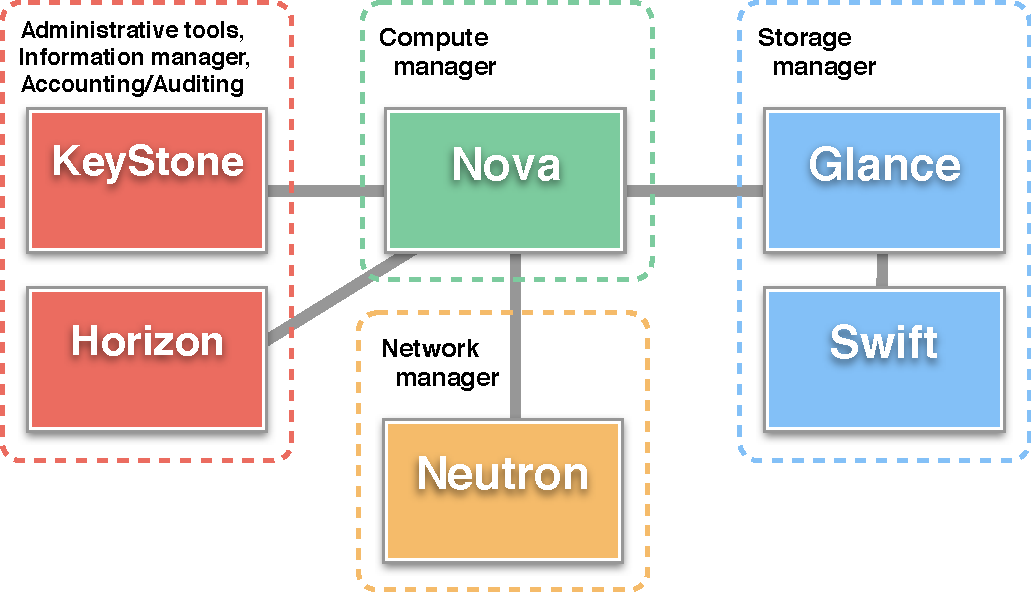
\includegraphics[width=7cm]{figures/OpenStack_architecture.pdf}
%\vspace*{-.3cm}
        \caption{Core-Services of OpenStack.}
        \label{fig:openstack}
%\vspace*{-.3cm}
\end{figure}


The OpenStack services are organized following the \textit{Shared Nothing} principle. Each instance of a service (\ie service worker) is exposed
through an API accessible through a \textit{Remote Procedure Call} (RPC) system implemented on top of a messaging queue or via web services
(REST). This enables a weak coupling between services. During their life-cycle, services create and manipulate logical objects that are persisted in
shared databases, thus enabling service workers to easily collaborate while keeping the compatibility with the \textit{Shared Nothing} principle.
 
%% \begin{itemize}
%%    \setlength{\itemsep}{0pt}
%%   \setlength{\parskip}{0pt}
%%    \setlength{\parsep}{0pt}
%% \item \textbf{A messaging queue}, implementing the AMQP protocal that enables
%% the collaboration between sub-services of a controller.
%% \item \textbf{A relational database} (DB) that stores inner states of a controller.
%% \end{itemize}

However, even if this organisation of services respects the \textit{Shared Nothing principle}, the message bus and the fact that objects are persisted
in shared databases limit the scalabilty of the system%a massively distributed infratructure based on OpenStack
, as stated in its documentation:

\begin{quote}
  \textit{OpenStack services support massive horizontal scale. Be aware that this is not the case for the entire supporting infrastructure. This is
    particularly a problem for the database management systems and message queues that OpenStack services use for data storage and remote procedure
    call communications.}
\end{quote}

As a consequence, the process of revising OpenStack towards a more decentralized and an advanced distributed functioning, should be carried out in
two ways: the distribution of the messaging queue and the distribution of the shared relational databases.

%%%
\subsection{Decentralizing the AMPQ Bus}

As indicated, services composing OpenStack collaborate mainly through a RPC system built on top of an AMQP bus. The AMQP implementation used by OpenStack
is \textit{RabbitMQ}. While this solution is generally articulated around the concept of a centralized master broker, it provides by default a cluster
mode that can be configured to work in a highly available mode. Several machines, each hosting a RabbitMQ instance, work together in an Active/Active
functioning where each queue is mirrored on all nodes. %This mode is recommended by the
%documentation  %for setting up  a multi-controller nodes OpenStack infrastructure.
While it has the advantage of being simple, it has the drawback of being very sensible to network latency, and thus it is not relevant for multi-site
configurations at large scale. This limitation is well known from the distributed messaging queue community. Few workarounds have been proposed for
solutions such as RabbitMQ and more recently, P2P-like systems such as ActiveMQ~\cite{activemq:2011} or ZeroMQ~\cite{zeromq:2013} have been released.
%. However as this limitation is well know from the
%distributed messaging queue community, we decided to not consider it as a major
%issue. First, few workarounds have been proposed for solutions such as RabbitMQ
%and more recently, P2P-like systems such as ActiveMQ~\cite{activemq:2011} and
%ZeroMQ~\cite{zeromq:2013} have been released.
Such broker-less solutions satisfy the LUC requirements in terms of scalability and because an action already showed that it is feasible to replace
RabbitMq with ZeroMQ\footnote{\url{https://wiki.openstack.org/wiki/ZeroMQ} (valid on Dec 2015)}, we chose to focus our efforts on the DB challenge.
% AMQP and scalabilty
% http://googlecloudplatform.blogspot.fr/2014/06/rabbitmq-on-google-compute-engine.html
% Performance evaluation of RESTful web services and AMQP protocol - http://ieeexplore.ieee.org/xpls/abs_all.jsp?arnumber=6614932&tag=1

%%%
\subsection{Decentralizing the Databases}

%% \begin{figure*}
%%   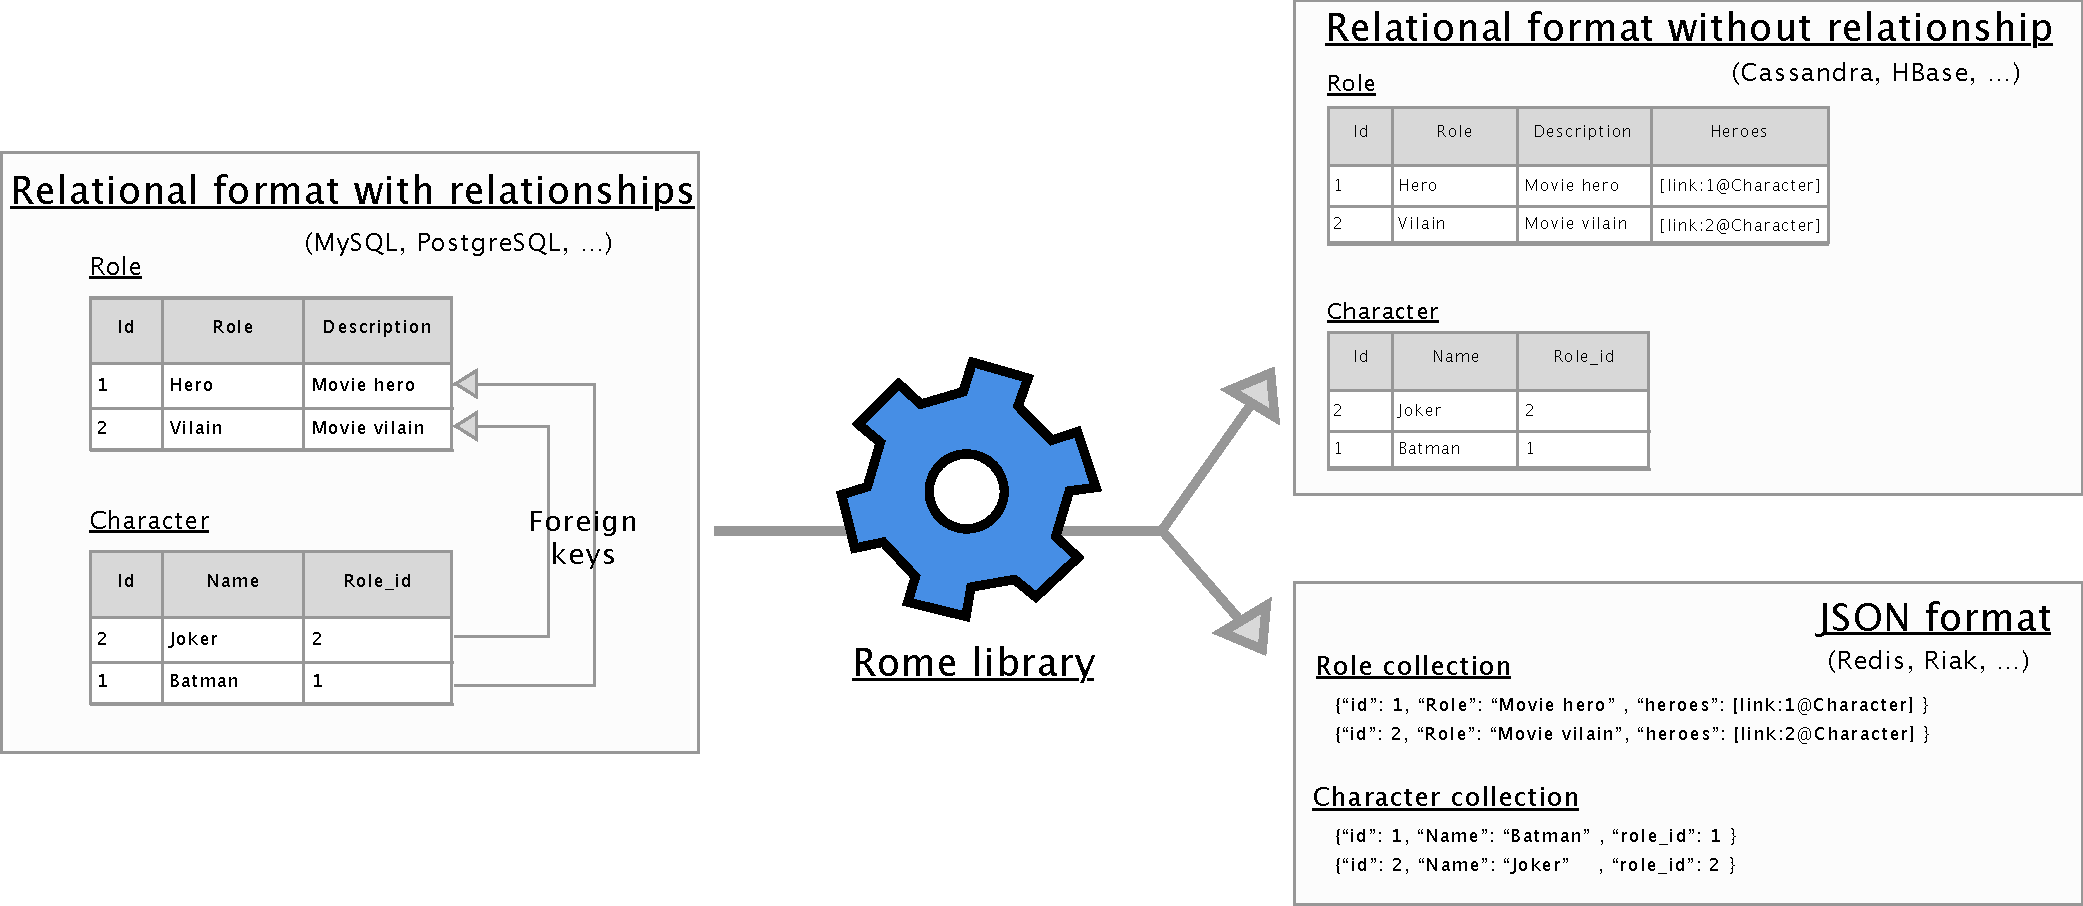
\includegraphics[width=.99\textwidth]{figures/rome_models.pdf}
%%   \caption{Rome is a library that enables to work with NoSQL databases with an object oriented interface.}
%%   \label{fig:rome_format}
%% \end{figure*}

From today's perspective, most of the OpenStack deployments are involving few compute nodes and do not require more than a single database (DB) node
in terms of scalability. Each instance of every service composing the OpenStack infrastructure can collaborate with remote instances by sharing
logical objects (inner-states) that are usually persisted in a single DB node.
%% Adrien: La phrase ci dessus est une redite et pourrait etre supprimé de mon point de vue
The use of a second DB is generally considered to satisfy the high availability constraint that is mandatory in production infrastructures. In such a
context, the OpenStack community recommends the use of at least an \textit{active/passive} replication strategy. A second DB acts as a failover of the
master instance. However, when the infrastructure becomes larger or includes distinct locations, it becomes mandatory to distribute the existing
relational DBs over several servers.% to address both challenges, \ie scalability and
%high-availability.
Two approaches are proposed by the OpenStack community.
%
The first one consists in partitioning the infrastructure into group called \emph{cells} configured as a tree. The top-cell is generally composed of
one or two nodes (\ie the top-cell does not include compute nodes) and is in charge of redistributing requests to the child cells. Each child cell can
be seen as an independent OpenStack deployment with its own DB server and message queue broker. In addition to facing hierarchical approach issues we
previously discussed (see Section~\ref{subsec:design-arg}), we highlight that additional mechanisms are mandatory on top of the vanilla OpenStack code
in order to make collaboration between cells possible. Consequently, this approach looks closer to a brokering solution than a native collaboration of
a IaaS management system as we target.
  %
The second approach consists in federating several OpenStack deployments throughout an \textit{active/active} replication
mechanism~\cite{kemme:vldb2010} provided by the \emph{Galera} solution. By such a mean, when an instance of a service processes a request and performs
some actions on one site, changes in the inner-states stored in the DB are also propagated to all the other DBs of the infrastructure. From a certain
point of view, it gives the illusion that there is only one unique DB shared by all OpenStack deployments. Although the described technique has been
used in production systems, most of them only involve a limited number of geographical sites. Indeed, active replication mechanisms imply important
overheads that limit the size of infrastructures.
  %
To sum up neither the hierarchical approach nor the active replication solution are suited to deal with a massively distributed infrastructure as the
one we target.

While not yet explored for the main OpenStack components, NoSQL databases seem to have more suitable properties for highly distributed context,
providing a better scalability and built-in replication mechanisms. Distributed Hash Tables (DHTs) and more recently key/value stores (KVSes) built on
top of the DHT concept such as \emph{Dynamo}~\cite{decandia:dynamo} have demonstrated their efficiency in terms of scalability and fault tolerance
properties. The challenge consists in analyzing how OpenStack internals can be revised to be able to manipulate inner-states through a KVS instead of
a classical SQL system. In the next section we present how we performed such a change for the Nova component.

%% \subsubsection{Rome library}

%% OpenStack doesn't  manipulate directly data  stored on the  relational database,
%% instead  it  uses  \textit{SQLAlchemy}  which serves  as  an  Object-Relationnal
%% mapping tool by  making the link between the relational  format used by database
%% and  the object  format used  by programs.  Thus OpenStack  services manipulates
%% inner-states stored in the database with an object oriented vision.

%% In light of this, we have developed a python library called \textit{``Rome"}
%% which targets at enabling python programs to manipulate data stored in NoSQL
%% databases with the same programmatic interfaces provided by \textit{SQLAlchemy}.
%% As there exists several types of NoSQL databases (Key/Values stores like Redis,
%% column oriented databases like Cassandra, ...), Rome supports several types of
%% databases, enabling to manipulate them with the same programmatic interfaces.

%% \textit{Rome} provides the support of relationships in NoSQL databases: 
%% relationships between tables are widely used in relational databases thanks to
%% the concept of foreign keys, and most of the NoSQL databases do not implement
%% this. \textit{Rome} support the definition of relationships between model
%% classes, and thus enables to propagate modifcation on an object to its linked
%% objects.

%% Moreover, \textit{Rome} implements the \textit{join} technic that enables to
%% combine rows of several tables, in the same manner as SQLAlchemy do. While
%% SQLAlchemy leverage the ``JOIN" operator in SQL language and thus delagate the
%% work to the database server, \textit{Rome} cannot do the same as most of the
%% NoSQL databases (REDIS, Cassandra) do not implement the ``JOIN" operation: this
%% operation is executed by ``ROME", on the client-side, thus maintaining the
%% compatibility with \textit{SQLAlchemy}.

%% Finally, \textit{Rome} enables the support of transactions as defined by
%% \textit{SQLAlchemy}: while \textit{SQLAlchemy} rely on transactional mechanisms
%% provided by database server, \textit{Rome} simulates this operation thanks to
%% a distributed lock implemented with \textit{REDIS} that enables to lock model
%% objects and use timeout measurement to detect deadlock situations.

%%%
\subsection{From MySQL to REDIS, The Nova POC\label{subsec:mysql-to-redis}}

As illustrated in Figure \ref{fig:nova_dbs}, the architecture of Nova has been organized in a way which ensures that each of its sub-services does not
directly manipulate the DB. Instead it calls API functions proposed by a service called ``nova-conductor''. This service forwards API calls to the
\textbf{``db.api''} component that proposes one implementation per database type. Currently, there is only one implementation that works on
relational DBs. This implementation relies on the \emph{SQLAlchemy} object-relational-mapping (ORM) that enables the manipulation of a relational
database via object oriented code.

\begin{figure}[htbp]
%\vspace*{-0.3cm}
        \centering
        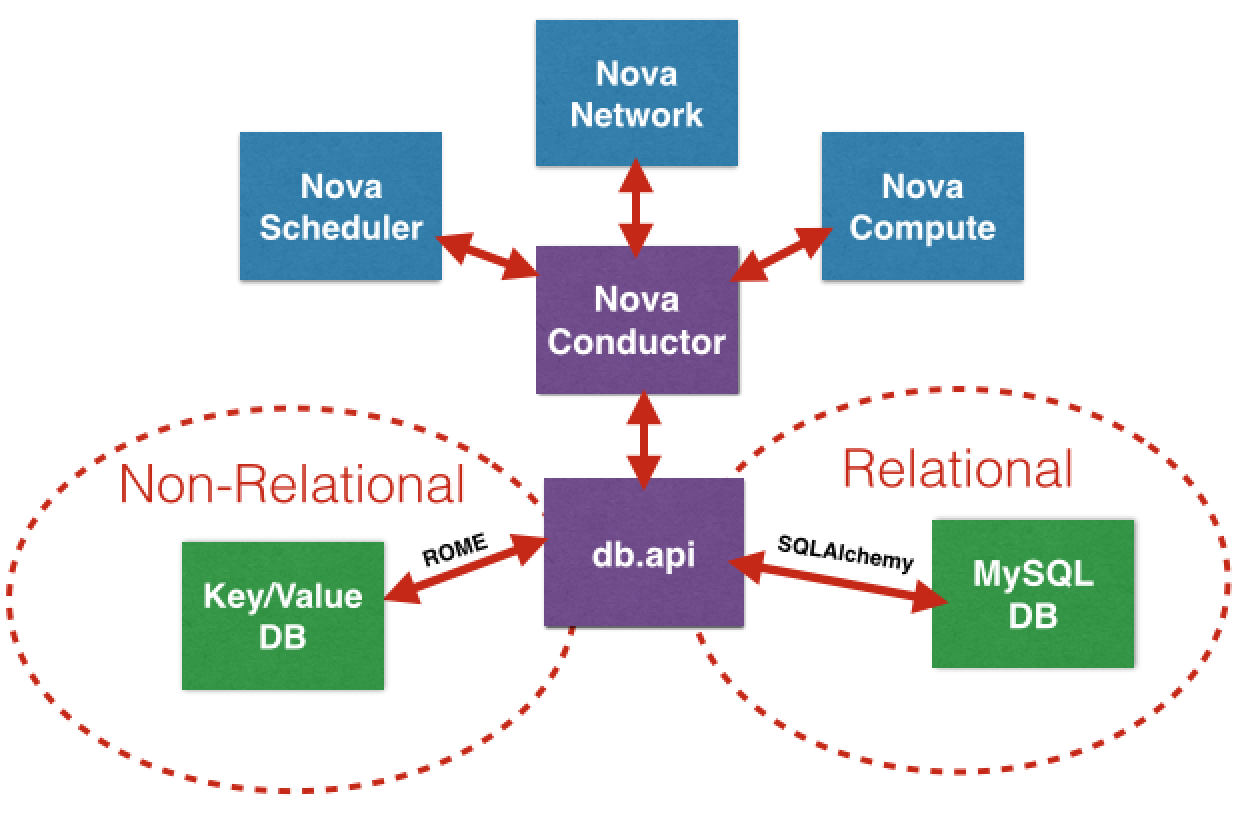
\includegraphics[width=8cm]{figures/rome_nova.png}
%\vspace*{-0.8cm}
        \caption{Nova - Software Architecture and DB dependencies.}
        \label{fig:nova_dbs}
%\vspace*{-.3cm}
\end{figure}

Thanks to the usage of this ORM, the given implementation is not tightly-coupled with the relational model. Such a feature enabled us to develop
\textit{ROME}, a library that exposes the same functions as \textit{SQLAlchemy} and performs the same actions but on non-relational DBs. As
\textit{ROME} and \textit{SQLAlchemy} are very similar, we have been able to copy the existing implementation of \textbf{``db.api''}, and to replace
every use of \textit{SQLAlchemy} by a call to \textit{ROME}, enabling Nova's services to work with a KVS, while limiting the number of changes in the
original source code.

Thanks to this modification, it is possible to deploy an OpenStack infrastructure that works with a natively distributed database, which gives a first
glimpse of large multi-site deployments. Figure~\ref{fig:newnova} depicts such a deployment:
%where the  OpenStack-Nova infrastructure is composed  of two
%kind of nodes: controller nodes (in charge of every aspect of the infrastructure) and
%compute nodes (dedicated to the hosting of VMs):
each geographical site hosts at least one controller node and at least a part of the NoSQL DB, \aka the KVS Controller nodes collaborate in a flat way
thanks to the shared KVS and the shared AMQP bus. The number of controller nodes on each site can vary according to the expected demand created by
end-users. Finally, a controller node can be deployed either on a dedicated node or be mutalized with a compute node as illustrated for Site 3. We
higlight that any controller node can provision VMs by orchestrating services on the whole infrastructure and not only on the site where it is
deployed. Concerning the choice of the NoSQL database, we chose to use REDIS in our prototype because of its deployment/usage simplicity. However we
are aware that databases that focus on high-availability and partition tolerance criteria, such as Cassandra~\cite{lakshman:2010}, could be a good fit
as they have already been deployed on production environments.

\begin{figure}[htbp]
        \centering
%        \vspace*{-.4cm}
%        \hspace*{-.2cm}
        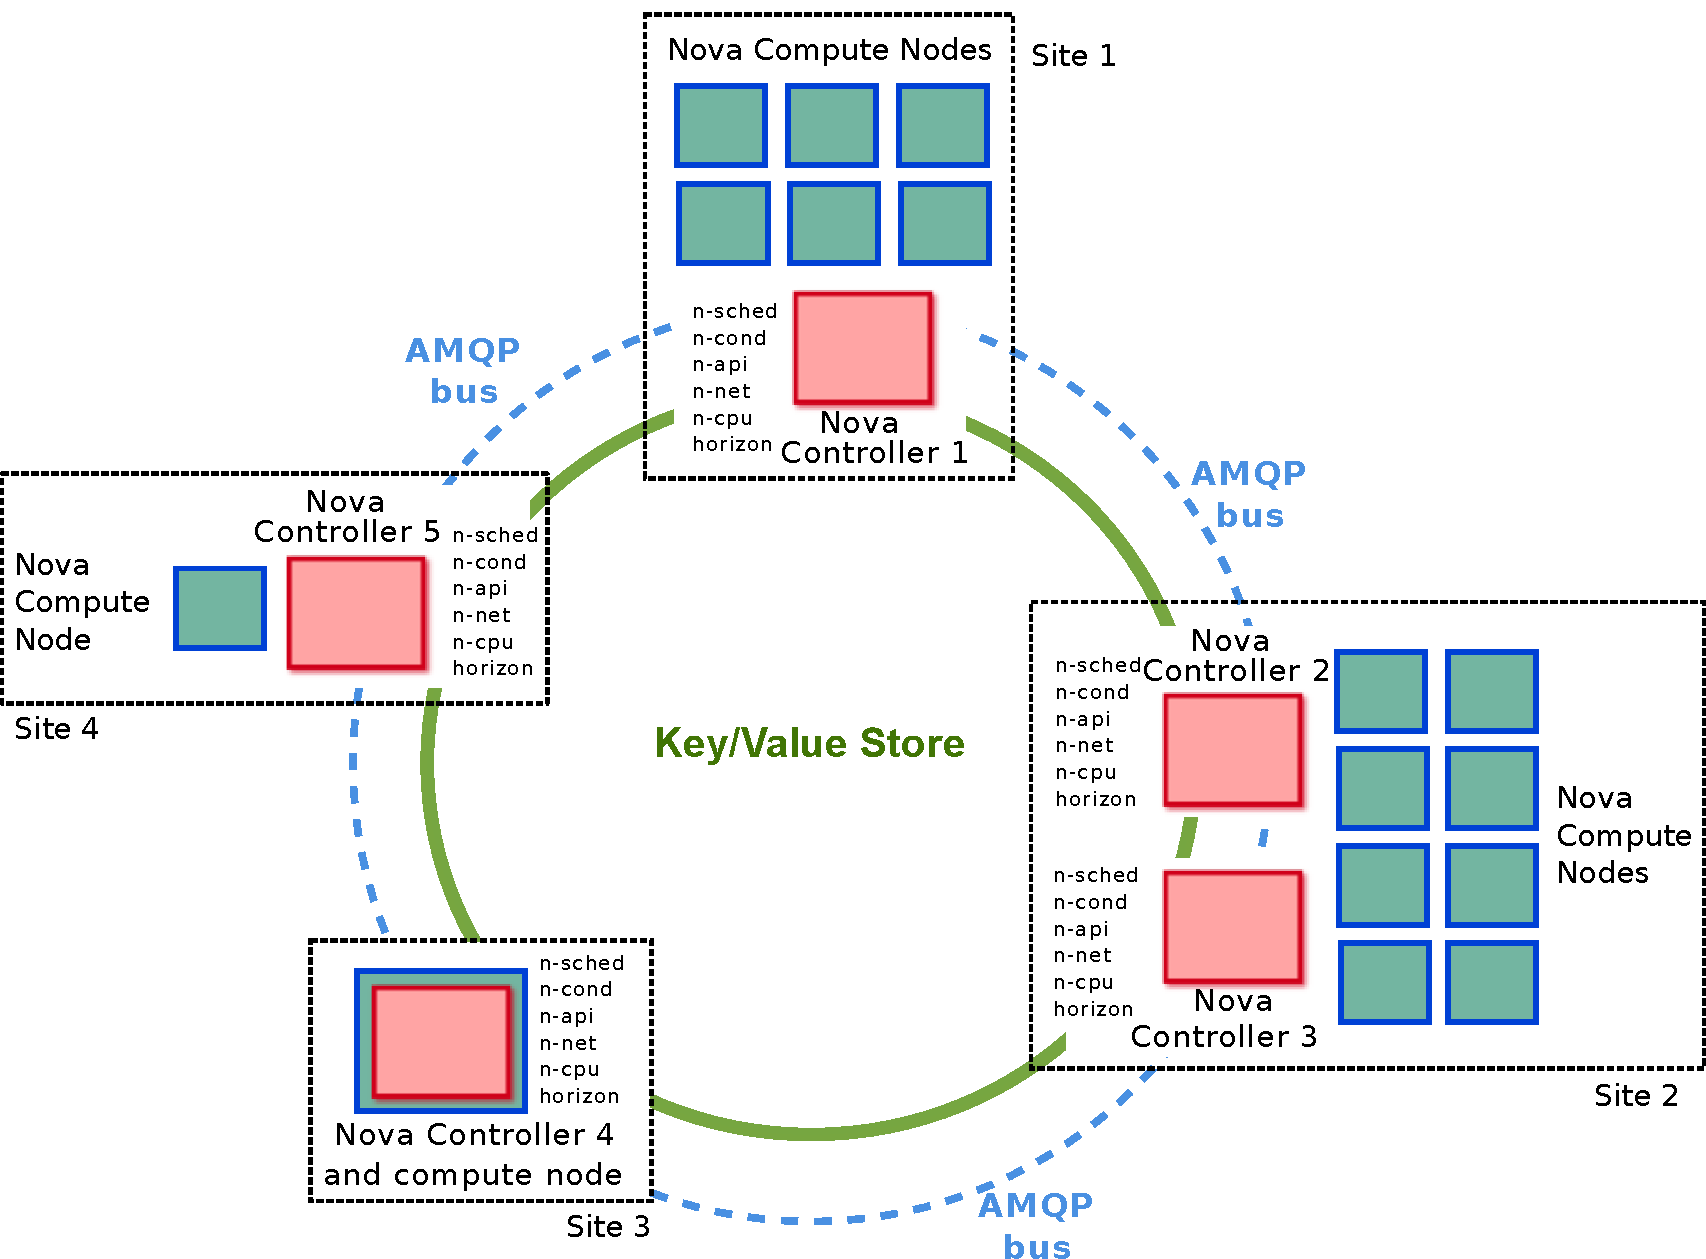
\includegraphics[width=.52\textwidth]{figures/OpenStack_distributed.pdf}
        \caption{Nova controllers (in light-red) are connected through a shared
          key/value backend and the AMQP bus. Each controller runs all nova
          services and can provision VMs on any compute node (in light blue).}
        \label{fig:newnova}
      %  \small{Each controller runs all nova services.}
%\vspace*{-.3cm}
\end{figure}


%% Our prototype  is under evaluation.  However, preliminary experiments  have been
%% performed  throughout 4  sites of  Grid'5000 including  12 compute  nodes and  4
%% controllers overall. While this infrastructure was rather small in comparison to
%% our target,  it aimed at  validating the interconnection of  several controllers
%% WANwide and  the correct  behaviour of  OpenStack using  our noSQL  backend. Our
%% prototype suceeded to provision 500 VMs in 300 seconds (each controller creating
%% 125 VMs  in parallel). A second  experiment validated the provisionning  of 2000
%% VMs  in less  than  30  min. We  are  currently  performing comparisons  between
%% OpenStack using  the historical MYSQL  backend \textit{v.s.,} using  a key/value
%% store backend.  Our goal  is to  validate that  manipulating internal  states of
%% Openstack through  a noSQL deliver performances  in the same order  of the MySQL
%% ones.
